\documentclass{article}
\usepackage{amsmath,amssymb}
\usepackage[numbers]{natbib}
\usepackage{geometry}
 \geometry{
 a4paper,
 total={170mm,257mm},
 left=30mm,
 top=30mm,
 right=30mm,
 bottom=30mm
 }
 
\usepackage{graphicx}
\usepackage{caption}
\usepackage{subcaption}
\usepackage{float}

\usepackage{multirow}
\usepackage{siunitx}
\usepackage{booktabs}
\usepackage{gensymb}

\setlength{\parskip}{1em}

\title{Reinforcement Learning Assignment-2 \\
	\Large Multi-Armed Bandit Problem \\}
\begin{document}
\author{Utkarsh Prakash \\ \normalsize 180030042}
\maketitle
\section{Problem Statement}
	A multi-armed Bandit is a set of distributions $\{\mathcal{R}_{a} | a \in \mathcal{A}\}$ where $\mathcal{A}$ is a known set of arms and $\mathcal{R}_{a}$ is the
	distribution of the rewards given the arm $a$. $K$ represents the number of arms being considered in the problem. At each time step, we select an arm 
	$A_{t} \in \mathcal{A}$ and get a reward $R_{t} \stackrel{}{\sim}
	\mathcal{R}_{A_{t}}$. Let $q(a)$ denote the expected reward that can be obtained if the arm $a$ is pulled, i.e. $q(a) = \mathbb{E}[R_{t} | A_{t} = a]$. Using,
	$q(a)$, we can define an optimal arm as the one having the highest value of $q(a)$. Let's denote the value $q(a)$ of this optimal arm as $v_{*}$. We can now 
	define regret for an action $a$ as $v_{*} - q(a)$. \par

	\noindent %The next paragraph is not indented
	The goal of the problem is to minimize the cummulative reward over fixed time (T), i.e.
	\begin{equation}
	\nonumber
		\min \sum_{n=1}^{T} (v_{*} - q(A_{n}))
	\end{equation}
\section{Experiment Setting}
	We consider Bernoulli and Normal Reward Distributions for our experiments. We sample the expected reward from a uniform distribution between [0, 1] for both the 
	reward distributions for each of the arm. We assume that the variance $(\sigma^{2})$ of the Normal reward distribution is known and we experiment with $\sigma^{2} = 0.1^{2}$ and
	$\sigma^{2} = 1^{2}$. \par
	
	\noindent %The next paragraph is not indented
	For each experiment we run our algorithm for 1000 time steps. This is considered to be a run for an algorithm with a given Bandit problem. In order to compare
	the performance of the algorithms fairly, in each run we evaluate the performance of the algorithm on the same Bandit problem. We run our algorithms for 1000
	runs with each run having a different Bandit problem. We use the following metrics for evaluating the performance of the algorithm:
	
	\begin{itemize}
		\item The total regret accumulated over time.
		\item The regret as a function of time.
		\item The percentage of plays in which the optimal arm is pulled.
		\item Average reward as a function of time.
	\end{itemize}
	
	Note that we average these metrics over 1000 runs of the algorithm. 
	
\section{Notations}
\begin{equation}
	x = \frac{\zeta}{t}
\label{default_schedule}
\end{equation}
\section{Bernoulli Reward Distribution}
	\subsection{K=2 arm Problem}
		\subsubsection{Greedy Algorithm}
		
		In this section, we compare the pure Greedy algorithm, $\epsilon$-greedy with fixed $\epsilon=0.1$ and $\epsilon=0.01$ and variable $\epsilon$ with the 
		following schedule:
		\begin{equation}
			\epsilon_{t} = min\{1, \frac{C}{t}\}
		\label{epsilon_greedy_schedule}
		\end{equation}
		where $C=10$ and $t$ is the total number of plays. We observe the following graphs:
		
		\begin{figure}[H]
		\graphicspath{ {../Experiments/Bernoulli_2_Greedy/} }
		\centering
		\begin{minipage}{.5\textwidth}
		  \centering
		  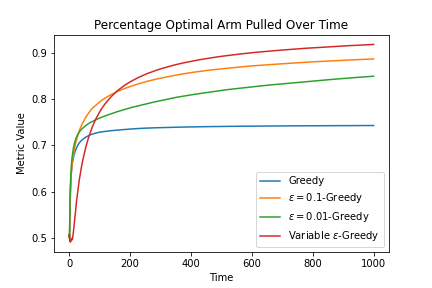
\includegraphics[width=\linewidth]{Percentage_Optimal_Arm_Pulled_Over_Time.png}
		  \captionof{figure}{Percentage Optimal Arm Pulled Over Time}
		  \label{fig:test1}
		\end{minipage}%
		\begin{minipage}{.5\textwidth}
		  \centering
		  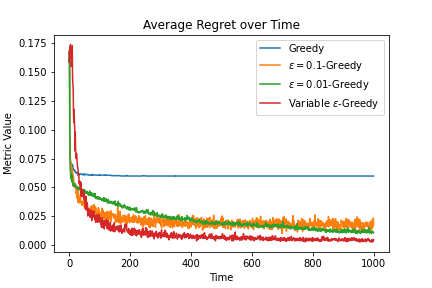
\includegraphics[width=\linewidth]{Average_Regret_over_Time.png}
		  \captionof{figure}{Average Regret over Time}
		  \label{fig:test2}
		\end{minipage}
		\end{figure}
		
		\textbf{Observations:}
		\begin{itemize}
			\item The variable $\epsilon$-Greedy tends to perform better than all of its counter-parts.
			\item In general, $\epsilon$-Greedy performs better than pure Greedy because of its tendency to explore the arms along with exploting the current 
				known knowledge.
		\end{itemize}
		
		
		\subsubsection{Softmax Policy}
		
		In this section, we compare the Softmax Policy which is defined as follows:
		\begin{equation}
		\nonumber
			\pi_{t}(a) = \frac{e^{q_{t}(a)/\tau}}{\sum_{i=1}^{K} e^{q_{t}(a_{i})/\tau}}
		\end{equation}
		where $\tau$ is the temperature hyperparameter. We compare the performance of Softmax Policy for $\tau=0.01$, $\tau=10000$ and variable $\tau$ with 
		schedule as defined in (\ref{default_schedule}) where $\zeta=10$. We reduce the $\tau$ overtime to control exploration-exploitation tradeoff. The graph for 
		different metrics are obtained as follows:
		
		\begin{figure}[H]
		\graphicspath{ {../Experiments/Bernoulli_2_Softmax/} }
		\centering
		\begin{minipage}{.5\textwidth}
		  \centering
		  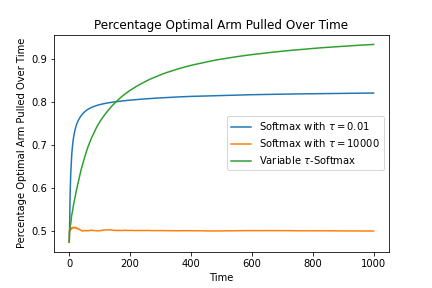
\includegraphics[width=\linewidth]{Percentage_Optimal_Arm_Pulled_Over_Time.png}
		  \captionof{figure}{Percentage Optimal Arm Pulled Over Time}
		  \label{fig:test1}
		\end{minipage}%
		\begin{minipage}{.5\textwidth}
		  \centering
		  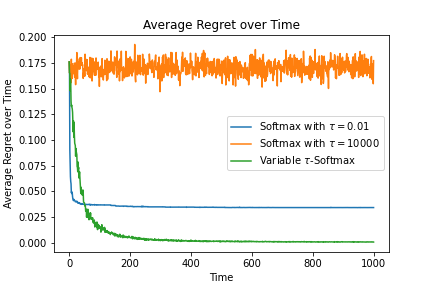
\includegraphics[width=\linewidth]{Average_Regret_over_Time.png}
		  \captionof{figure}{Average Regret over Time}
		  \label{fig:test2}
		\end{minipage}
		\end{figure}
		
		\textbf{Observations:}
		\begin{itemize}
			\item For small values of $\tau=0.01$, the algorithm performs poorly because in the limit when $\tau \to 0$, then the algorithm performs greedily.
			\item For large values of $\tau=10,000$, the algorithm performs poorly because in the limit when $\tau \to \infty$, then the algorithm picks an arm
				uniformly at random. Therefore, for such large values of $\tau$ the algorithm explores at lot.
			\item The variable $\tau$-Softmax tends to perform better than all of its counter-parts. This is because earlier when the value of $\tau$ is high, we
			tend to explore more, whereas as time progresses and we gather knowledge of different arms, we reduce the value of $\tau$ so as to exploit the knowledge
			that we have gathered (i.e., pull the arm which has highest estimated average reward with high probability).
		\end{itemize}
		
		
		\subsubsection{UCB Algorithm}
		In this section we compare the UCB algorithm where we pick the arm which has the highest value of 
		\begin{equation}
		\nonumber
			\arg max_{a \in \mathcal{A}} \left (q_{t}(a) + C\sqrt{\frac{2 \ln t}{n_{t}(a)}} \right )
		\end{equation}
		where $C$ is a hyperparameter which controls exploration-exploitation tradeoff. We used three different values of $C$ (1, 100 and variable). The graphs 
		obtained are as follows:
		
		\begin{figure}[H]
		\graphicspath{ {../Experiments/Bernoulli_2_UCB/} }
		\centering
		\begin{minipage}{.5\textwidth}
		  \centering
		  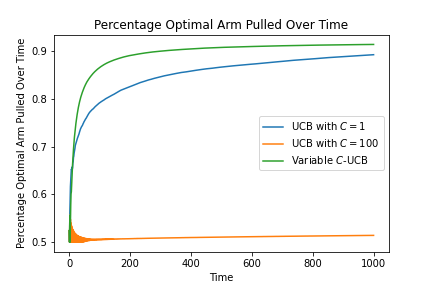
\includegraphics[width=\linewidth]{Percentage_Optimal_Arm_Pulled_Over_Time.png}
		  \captionof{figure}{Percentage Optimal Arm Pulled Over Time}
		  \label{fig:test1}
		\end{minipage}%
		\begin{minipage}{.5\textwidth}
		  \centering
		  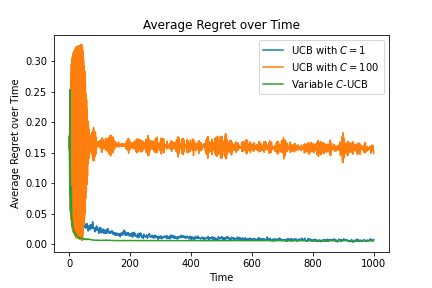
\includegraphics[width=\linewidth]{Average_Regret_over_Time.png}
		  \captionof{figure}{Average Regret over Time}
		  \label{fig:test2}
		\end{minipage}
		\end{figure}
		
		\textbf{Observations:}
		\begin{itemize}
			\item We can see the variable-$C$-UCB algorithm outperforms its counter-parts.
			\item For large values of $C=100$, the algorithm performs poorly because it explores too much.
		\end{itemize}
		
		\subsubsection{Thompson Sampling}
		In Thompson Sampling, we maintain a Beta distribution prior over $q_{t}(a)$. We sample a value $Q_{t}(a)$ from this Beta distribution for each arm, i.e.
		$q_{t}(a) \stackrel{}{\sim} Q_{t}(a)$. Now, we select the arm which has the highest value of $Q_{t}(a)$. The results obtained for this algorithm is as 
		follows:
		
		\begin{figure}[H]
		\graphicspath{ {../Experiments/Bernoulli_2_Thompson_Sampling/} }
		\centering
		\begin{minipage}{.5\textwidth}
		  \centering
		  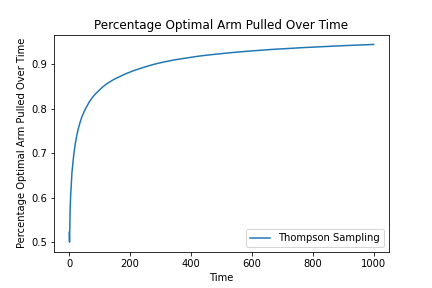
\includegraphics[width=\linewidth]{Percentage_Optimal_Arm_Pulled_Over_Time.png}
		  \captionof{figure}{Percentage Optimal Arm Pulled Over Time}
		  \label{fig:test1}
		\end{minipage}%
		\begin{minipage}{.5\textwidth}
		  \centering
		  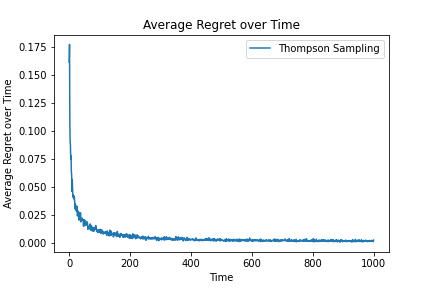
\includegraphics[width=\linewidth]{Average_Regret_over_Time.png}
		  \captionof{figure}{Average Regret over Time}
		  \label{fig:test2}
		\end{minipage}
		\end{figure}
		
		\subsubsection{Reinforce Algorithm}
		The reinforce algorithm follows the following policy:
		\begin{equation}
		\nonumber
			\pi_{t}(a) = \frac{e^{\theta_{t}(a)}}{\sum_{i=1}^{K} e^{\theta_{t}(a_{i})}}
		\end{equation}
		where $\theta_{t}(a)$ are the learnable parameters of the algorithm. These parameters can be learned using Stochastic Gradient Ascent with the following
		update rule:
		\begin{equation}
		\nonumber
			\theta_{t}(a) = \begin{cases}
				\theta_{t}(A_{t}) + \alpha (R_{t} - b) (1 - \pi_{t}(A_{t})) & if a = A_{t} \\
				\theta_{t}(a) + \alpha (R_{t} - b) \pi_{t}(a) & if a \ne A_{t}
			\end{cases}
		\end{equation}
		where $b$ is a baseline and is generally chosen to be the average of all the rewards up through and including time t. The following graphs were obtained
		with and without baselines:
		
		\begin{figure}[H]
		\graphicspath{ {../Experiments/Bernoulli_2_Reinforce/} }
		\centering
		\begin{minipage}{.5\textwidth}
		  \centering
		  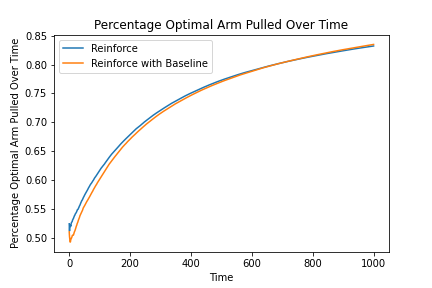
\includegraphics[width=\linewidth]{Percentage_Optimal_Arm_Pulled_Over_Time.png}
		  \captionof{figure}{Percentage Optimal Arm Pulled Over Time}
		  \label{fig:test1}
		\end{minipage}%
		\begin{minipage}{.5\textwidth}
		  \centering
		  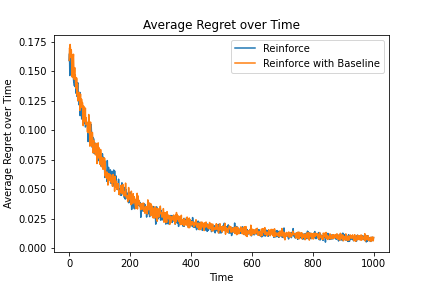
\includegraphics[width=\linewidth]{Average_Regret_over_Time.png}
		  \captionof{figure}{Average Regret over Time}
		  \label{fig:test2}
		\end{minipage}
		\end{figure}
		
		\textbf{Observations:}
		\begin{itemize}
			\item We really don't see any difference in performance between the algorithm with and without baselines.
		\end{itemize}
		
		\subsubsection{Comparison of all Algorithms}
		\label{2_bernoulli_comparison}
		In this section we compare the performance of all the algorithms for the 2 arm problem. We pick the best performing variation of the algorithm as found
		in the above experiments for comparison i.e. the following algorithms were used comparison:
		\begin{itemize}
			\item Variable $\epsilon$-Greedy where $\epsilon$ decreases according to the schedule defined in (\ref{epsilon_greedy_schedule}) with $C=10$.
			\item Variable $\tau$-Softmax where $\tau$ decreases according to the schedule defined in (\ref{default_schedule}) with $\zeta=10$.
			\item Variable $C$-UCB where $C$ decreases according to the schedule defined in (\ref{default_schedule}) with $\zeta=10$.
			\item Thompson Sampling Algorithm
			\item Reinforce Algorithm without baseline. This was chosen since we didn't find any considerable improvement in the performance by using baseline.
		\end{itemize}
		
		The results obtained are as follows:
		
		\begin{figure}[H]
		\graphicspath{ {../Experiments/Bernoulli_2_All/} }
		\centering
		\begin{minipage}{.5\textwidth}
		  \centering
		  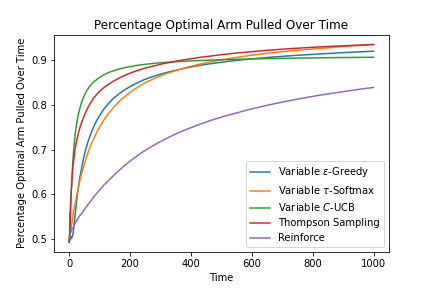
\includegraphics[width=\linewidth]{Percentage_Optimal_Arm_Pulled_Over_Time.png}
		  \captionof{figure}{Percentage Optimal Arm Pulled Over Time}
		  \label{fig:test1}
		\end{minipage}%
		\begin{minipage}{.5\textwidth}
		  \centering
		  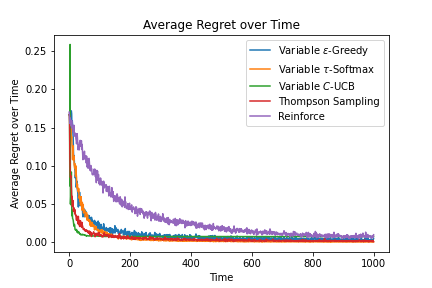
\includegraphics[width=\linewidth]{Average_Regret_over_Time.png}
		  \captionof{figure}{Average Regret over Time}
		  \label{fig:test2}
		\end{minipage}
		\end{figure}
		
		\begin{figure}[H]
		\graphicspath{ {../Experiments/Bernoulli_2_All/} }
		\centering
		\begin{minipage}{.5\textwidth}
		  \centering
		  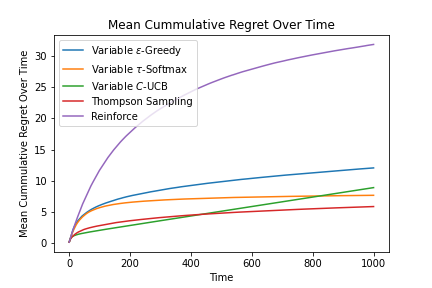
\includegraphics[width=\linewidth]{Mean_Cummulative_Regret_Over_Time.png}
		  \captionof{figure}{Percentage Optimal Arm Pulled Over Time}
		  \label{fig:test1}
		\end{minipage}%
		\begin{minipage}{.5\textwidth}
		  \centering
		  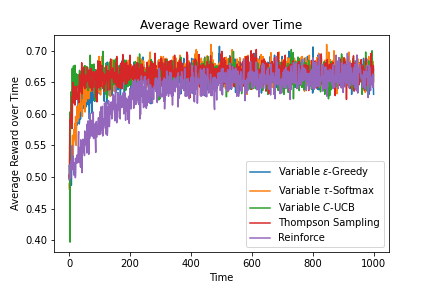
\includegraphics[width=\linewidth]{Average_Reward_over_Time.png}
		  \captionof{figure}{Average Regret over Time}
		  \label{fig:test2}
		\end{minipage}
		\end{figure}
		
		\textbf{Observations:}
		\begin{itemize}
			\item Variable $\epsilon$-Greedy, Variable $\tau$-Softmax, Variable $C$-UCB and Thompson Sampling algorithm seems to perform equally well. This means
				that any algorithm which optimally trades-off between exploration and exploitation, should perform well i.e. have logarithmic cummalative regret over 
				time. This is an interesting observation as simple algorithms with simple heuristics tend to perform at par with other algorithms with more 
				sophisticated heuristics.
			\item Reinforce algorithm doesn't tend to perform that well when compared to its counter-parts. If we look at the plot for the average regret over time
				for Reinforce algorithm, we find that it intially decreases very slowly. However, later it reaches the same level as that of other algorithms. This
				nature can be attributed to the fact that the parameters of the algorithm are learned slowly. Thereby, by increasing the learning rate for the 
				stochastic gradient ascent may fix the problem and the performance can become at par with other algorithms.	
		\end{itemize}
		
	\subsection{K=5 arm Problem}
		\label{5_bernoulli_comparison}
		We repeated similar experiments for each of the algorithm as we did for $K=2$ arm case to find the best performing variant of an algorithm. We found the 
		graphs to be following a similar trend as for $K=2$ case, therefore, we do not include them in our report. We then compared each of these best performing
		algorithms i.e. we compared the performance of the following algorithms for $K=5$ arms:
		\begin{itemize}
			\item Variable $\epsilon$-Greedy where $\epsilon$ decreases according to the schedule defined in (\ref{epsilon_greedy_schedule}) with $C=10$.
			\item Variable $\tau$-Softmax where $\tau$ decreases according to the schedule defined in (\ref{default_schedule}) with $\zeta=10$.
			\item Variable $C$-UCB where $C$ decreases according to the schedule defined in (\ref{default_schedule}) with $\zeta=10$.
			\item Thompson Sampling Algorithm
			\item Reinforce Algorithm without baseline. This was chosen since we didn't find any considerable improvement in the performance by using baseline.
		\end{itemize}
		
		The results obtained are as follows:
		
		\begin{figure}[H]
		\graphicspath{ {../Experiments/Bernoulli_5_All/} }
		\centering
		\begin{minipage}{.5\textwidth}
		  \centering
		  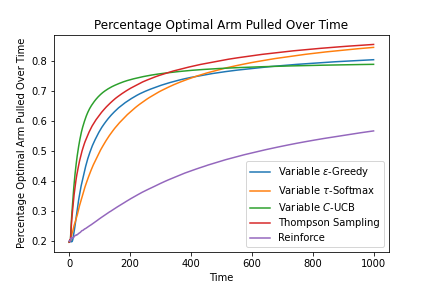
\includegraphics[width=\linewidth]{Percentage_Optimal_Arm_Pulled_Over_Time.png}
		  \captionof{figure}{Percentage Optimal Arm Pulled Over Time}
		  \label{fig:test1}
		\end{minipage}%
		\begin{minipage}{.5\textwidth}
		  \centering
		  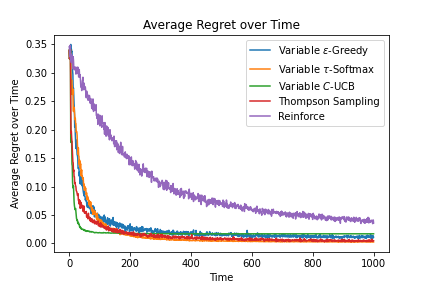
\includegraphics[width=\linewidth]{Average_Regret_over_Time.png}
		  \captionof{figure}{Average Regret over Time}
		  \label{fig:test2}
		\end{minipage}
		\end{figure}
		
		\begin{figure}[H]
		\graphicspath{ {../Experiments/Bernoulli_5_All/} }
		\centering
		\begin{minipage}{.5\textwidth}
		  \centering
		  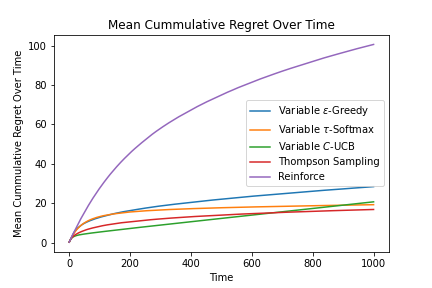
\includegraphics[width=\linewidth]{Mean_Cummulative_Regret_Over_Time.png}
		  \captionof{figure}{Percentage Optimal Arm Pulled Over Time}
		  \label{fig:test1}
		\end{minipage}%
		\begin{minipage}{.5\textwidth}
		  \centering
		  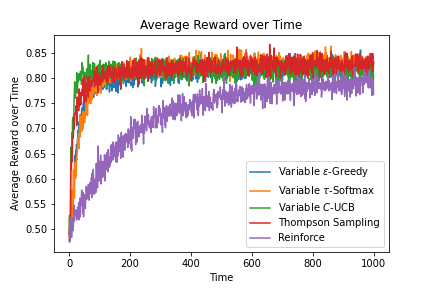
\includegraphics[width=\linewidth]{Average_Reward_over_Time.png}
		  \captionof{figure}{Average Regret over Time}
		  \label{fig:test2}
		\end{minipage}
		\end{figure} 
		
		Since, the trends in the graphs are similar to $K=2$ case, we defer the further discussion on the results to the section \ref{bernoulli_comparison}  where we compare
		the relative performance of the algorithm for different number of arms.
		
	\subsection{K=10 arm Problem}
		\label{10_bernoulli_comparison}
		We repeated similar experiments for each of the algorithm as we did for $K=2$ arm case to find the best performing variant of an algorithm. We found the 
		graphs to be following a similar trend as for $K=2$ case, therefore, we do not include them in our report. We then compared each of these best performing
		algorithms i.e. we compared the performance of the following algorithms for $K=10$ arms:
		\begin{itemize}
			\item Variable $\epsilon$-Greedy where $\epsilon$ decreases according to the schedule defined in (\ref{epsilon_greedy_schedule}) with $C=10$.
			\item Variable $\tau$-Softmax where $\tau$ decreases according to the schedule defined in (\ref{default_schedule}) with $\zeta=10$.
			\item Variable $C$-UCB where $C$ decreases according to the schedule defined in (\ref{default_schedule}) with $\zeta=10$.
			\item Thompson Sampling Algorithm
			\item Reinforce Algorithm without baseline. This was chosen since we didn't find any considerable improvement in the performance by using baseline.
		\end{itemize}
		
		The results obtained are as follows:
		
		\begin{figure}[H]
		\graphicspath{ {../Experiments/Bernoulli_10_All/} }
		\centering
		\begin{minipage}{.5\textwidth}
		  \centering
		  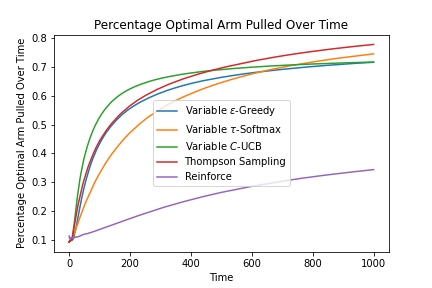
\includegraphics[width=\linewidth]{Percentage_Optimal_Arm_Pulled_Over_Time.png}
		  \captionof{figure}{Percentage Optimal Arm Pulled Over Time}
		  \label{fig:test1}
		\end{minipage}%
		\begin{minipage}{.5\textwidth}
		  \centering
		  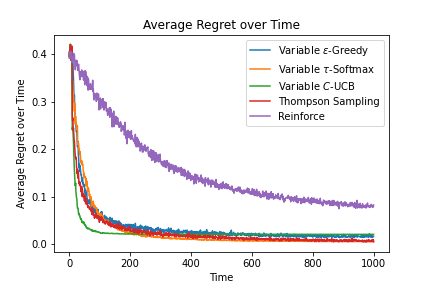
\includegraphics[width=\linewidth]{Average_Regret_over_Time.png}
		  \captionof{figure}{Average Regret over Time}
		  \label{fig:test2}
		\end{minipage}
		\end{figure}
		
		\begin{figure}[H]
		\graphicspath{ {../Experiments/Bernoulli_10_All/} }
		\centering
		\begin{minipage}{.5\textwidth}
		  \centering
		  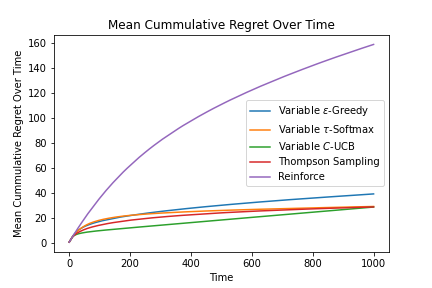
\includegraphics[width=\linewidth]{Mean_Cummulative_Regret_Over_Time.png}
		  \captionof{figure}{Percentage Optimal Arm Pulled Over Time}
		  \label{fig:test1}
		\end{minipage}%
		\begin{minipage}{.5\textwidth}
		  \centering
		  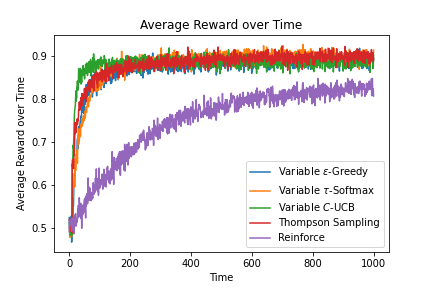
\includegraphics[width=\linewidth]{Average_Reward_over_Time.png}
		  \captionof{figure}{Average Regret over Time}
		  \label{fig:test2}
		\end{minipage}
		\end{figure} 
		
		Since, the trends in the graphs are similar to $K=2$ case, we defer the further discussion on the results to the section \ref{bernoulli_comparison} where we compare
		the relative performance of the algorithm for different number of arms.
		
	\subsection{Comparison of algorithms for different number of arms}
		\label{bernoulli_comparison}
		The following table lists the cummalative regret at the end of 1000 plays averaged over 1000 runs:
		
		\begin{table}[H]
		  \begin{tabular}{lSSSS}
			\toprule
			\multirow{1}{*}{\textbf{Algorithms}} &
			  \multicolumn{1}{c}{\textbf{K=2 Arms}} &
			  \multicolumn{1}{c}{\textbf{K=5 Arms}} &
			  \multicolumn{1}{c}{\textbf{K=10 Arms}} \\
			  % & {\textbf{Learned angle}} & {\textbf{Test Accuracy}} & {\textbf{Learned angle}} & {\textbf{Test Accuracy}} \\
			  \midrule
			Variable $\epsilon$-Greedy & 12.07 & 28.48 & 39.04  \\
			Variable $\tau$-Softmax & 7.68 & 19.32 & 28.97   \\
			Variable $C$-UCB & 8.91 & 20.77 & 28.52   \\
			Thompson Sampling & 5.87 & 16.89 & 28.58   \\
			Reinforce Algorithm (without baseline) & 31.88 & 100.61 & 158.87   \\
			\bottomrule
		  \end{tabular}
		  \caption{Comparison of cummalative regret of different algorithms for different number of arms for 1000 plays averaged over 1000 runs.}
		\end{table}
		
		One thing to note is that we used the same hyperparameters for different number of arms in order to facilitate fair comparison between the performance
		of the algorithms. The above table and the plots of section \ref{2_bernoulli_comparison}, \ref{5_bernoulli_comparison} and \ref{10_bernoulli_comparison} highlights that the 
		performance of all the algorithms decreases considerably as the number of arms are increased. However, the relative order of performance between algorithms
		remain as it is. We observe similar trends for other metrics as well.
		
		
		\begin{equation}
		\nonumber
		\end{equation}
		
		\begin{itemize}
			\item
		\end{itemize}
\end{document}